\documentclass{standalone}
\usepackage{tikz}

\begin{document}

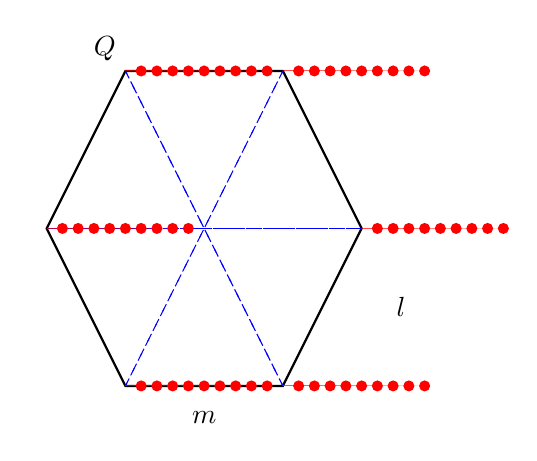
\begin{tikzpicture}[scale=2]
    % Define coordinates of the vertices of the hexagon
    \coordinate (A) at (0, 1);
    \coordinate (B) at (1, 1);
    \coordinate (C) at (1.5, 0);
    \coordinate (D) at (1, -1);
    \coordinate (E) at (0, -1);
    \coordinate (F) at (-0.5, 0);

    % Draw the hexagon
    \draw[thick] (A) -- (B) -- (C) -- (D) -- (E) -- (F) -- cycle;

    % Draw dashed lines from each vertex to the opposite side
    \draw[dashed, blue] (A) -- (D);
    \draw[dashed, blue] (B) -- (E);
    \draw[dashed, blue] (C) -- (F);
    \draw[dashed, blue] (D) -- (A);
    \draw[dashed, blue] (E) -- (B);
    \draw[dashed, blue] (F) -- (C);

    % Mark points on the dashed lines
    \foreach \x in {0.1, 0.2, ..., 0.9} {
        \fill[red] (A) -- ++(\x, 0) circle (1pt);
        \fill[red] (B) -- ++(\x, 0) circle (1pt);
        \fill[red] (C) -- ++(\x, 0) circle (1pt);
        \fill[red] (D) -- ++(\x, 0) circle (1pt);
        \fill[red] (E) -- ++(\x, 0) circle (1pt);
        \fill[red] (F) -- ++(\x, 0) circle (1pt);
    }

    % Label the vertices
    \node at (A) [above left] {$Q$};
    \node at (B) [above right] {};
    \node at (C) [right] {};
    \node at (D) [below right] {};
    \node at (E) [below left] {};
    \node at (F) [left] {};

    % Label the sides
    \node at (0.5, -1.2) {$m$};
    \node at (1.75, -0.5) {$l$};
\end{tikzpicture}

\end{document}